% Also check out Professor Matloff's guide: 
% http://heather.cs.ucdavis.edu/~matloff/LaTeX/HowToCreate.html.
\documentclass{article}

% Packages Used
\usepackage{fancyhdr} % Required for custom headers
\usepackage{lastpage} % Required to determine the last page for the footer
\usepackage{extramarks} % Required for headers and footers
\usepackage{graphicx} % Required to insert images
\usepackage{lipsum} % Used for inserting dummy 'Lorem ipsum' text into the template
\usepackage{comment}  % Used for multi-line commenting
\usepackage{booktabs} % For better looking tables
\usepackage{array}       % for better arrays (eg matrices) in maths
\usepackage{paralist}    % very flexible & customisable lists (eg. enumerate/itemize, etc.)
\usepackage{verbatim}  % adds environment for commenting out blocks of text & for better verbatim
\usepackage{subfig}      % make it possible to include more than one captioned figure/table in a single float
\usepackage{amsthm}   % make proofs look better
\usepackage{amsfonts}
\usepackage{amsmath}
\usepackage{amssymb}
\usepackage{eufrak}      % for fraktur fonts
\usepackage{mathabx}  % for \divides
\usepackage{enumerate} % to get lists enumerated with letters
\usepackage{hyperref}  % to get attractive URLs
\usepackage{bussproofs} % for setting proofs
\usepackage{etoolbox}
\usepackage{enumitem}
\usepackage{tabularx}
%algorithm
\usepackage{algorithmicx}
\usepackage[ruled]{algorithm}
\usepackage{algpseudocode}
\usepackage{algpascal}
\usepackage{algc}
\usepackage{tikz}
\usepackage{tikz-qtree}
%\algdisablelines
\newcommand{\alg}{\texttt{algorithmicx}}
\newcommand{\old}{\texttt{algorithmic}}
\newcommand{\euk}{Euclid}
\newcommand\ASTART{\bigskip\noindent\begin{minipage}[b]{0.5\linewidth}}
\newcommand\ACONTINUE{\end{minipage}\begin{minipage}[b]{0.5\linewidth}}
\newcommand\AENDSKIP{\end{minipage}\bigskip}
\newcommand\AEND{\end{minipage}}


% For theorem enviornment
\theoremstyle{definition}
\newtheorem{definition}{Definition}
\newtheorem{theorem}{Theorem}[section]
\newtheorem{corollary}{Corollary}[theorem]
\newtheorem{lemma}{Lemma}

\newtheorem{mathrule}{Rule}
\newtheorem{case}{Case}
\newtheorem{subcase}{Case}[case]

\theoremstyle{plain}
\newtheorem{example}{Example}
\newtheorem{problem}{Problem}[section]
\providecommand{\ceil}[1]{\left \lceil #1 \right \rceil }
\providecommand{\floor}[1]{\left \lfloor #1 \right \rfloor }
% For improved end of proof formatting
\patchcmd{\endproof}  % <cmd>
  {\endtrivlist}               % <search>
  {\endtrivlist\par\nobreak\vspace*{\dimexpr-\baselineskip-\parskip}\nobreak\noindent\hrulefill}% <replace>
  {}{}                            % <succes><failure>

% Margins
\topmargin=-0.45in
\evensidemargin=0in
\oddsidemargin=0in
\textwidth=6.5in
\textheight=9.0in
\headsep=0.25in 

\linespread{1.1} % Line spacing

% Set up the header and footer
\pagestyle{fancy}
\lhead{ECS20: Discrete Mathematics\\ UC Davis - Patrice Koehl} % Top left header
\chead{} % Top center header
\rhead{\firstxmark Anze Wang ID: 912777492\\ECS 020 A03} % Top right header
\lfoot{\lastxmark} % Bottom left footer
\cfoot{} % Bottom center footer
\rfoot{Page\ \thepage\ of\ \pageref{LastPage}} % Bottom right footer

\setlength\parindent{10pt} % Removes all indentation from paragraphs

% Common boolean operators.
%\newcommand*\AND{\wedge}
%\newcommand*\OR{\vee}
%\newcommand*\NOT{\neg}
%\newcommand*\IMPLIES{\implies}
%\newcommand*\XOR{\mathbin{\oplus}}


\begin{document}

\begin{center} \bf \LARGE Homework 8\\
\end{center}


\begin {enumerate}[itemindent=30pt,label=\bf Exercise {\arabic*}:]
\item .\\
How many strings are there of four lower case letters that have the letter x in them?
\subitem Number of strings of length $4$ $=26^4$
\subitem Number of strings of length $4$ other than $x$ $=25^4$
\subitem Thus, the answer is $26^4 - 25^4= 66351$ strings.
\item. \\How many strings of four decimal digits
\subitem a)do not contains the same digit twice?$$10*9*8*7 = 5040 $$ 
\subitem b)End with an even digit?$$ 10^3*5 = 5000$$
\subitem c)Have exactly three digits that are $9$s?$$9*4 = 36$$
\item .\\How many license plates can be made using either three digits followed by three letters, or three letters followed by three digits?
$$ 9^3*26^3 + 26^3*9^3 = 2(26^3*9^3) = 25625808$$
\item .\\How many subsets of a set with $100$ elements have more than one element?
\subitem All of the subset $=2^{100}$
\subitem The sub set has less than one element $=100+1$
\subitem Thus, the answer is $2^{100} - 100 -1$.
\item .\\How many bit strings of length 10 contain either five consecutive 0s or five consecutive 1s?
\subitem let's consider 5 consecutive 1s first:
\subitem if it start at position 1, remaining digits can be both $1$ and $0$: $2^5 = 32$
\subitem if it start at position $k = 2,3,4,5,6$, the number at position $k-1$ must be o, or it will be in previous cases: $5*2^4$
\subitem So the total number is $2^5 + 5*2^4 = 112$
\subitem 5 consecutive 0s is similar as 5 consecutive 1s, so we get another $112$.
\subitem because we count $0000011111$ and $1111100000$ twice, we should subtract 2 from the answer.
\subitem Thus the final answer is $112*2 -2 = 222$
\newpage
\item. \\ Use a tree diagram to find the number of bit strings of length four with no three consecutive $0$s.
\begin{center}
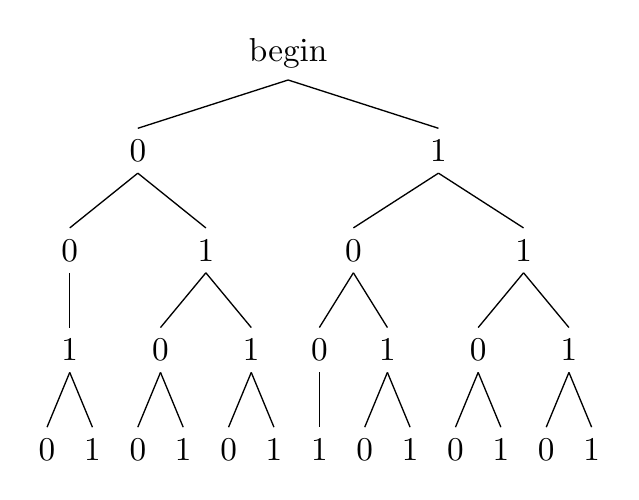
\begin{tikzpicture}[scale = 1.2]
\Tree
[.begin [.0 [.0 [.1 [.0 ] [.1 ] ] ] [.1 [.0 	[.0 ] [.1 ] ] [.1 [.0 ] [.1 ] ] ] ] [.1 [.0 [.0 [.1 ] ] [.1 [.0 ] [.1 ] ] ] [.1 [.0 [.0 ] [.1 ] ] [.1 [.0 ] [.1 ] ] ] ] ]
\end{tikzpicture}
\end{center}
\subitem So there are $13$ strings of length four with no three consecutive $0$s.
\item .\\Form a group of 13 men, 8 women, 2 boys and 4 girls.
\subitem (a)How many ways can a man, a woman, a boy and a girl be selected? $$13*8*2*4 = 832$$
\subitem (b)How many ways can a male and a female be selected?
$$(13+2)*(8+4) = 180$$
\subitem (c)How many ways can a person be selected?
$$13+8+2+4 = 27$$
\item Extra Credit
\subitem How many numbers in the range 100-999 have no repeated digits? (For example, $110$ and $211$ have repeated $1$, while $101$ is OK) $$9*9*9 = 729$$
\subitem Now how many of them are even? (be careful!).
\subitem \qquad if the first digit is even, the second is odd $$4*5*5 = 100$$
\subitem \qquad if the first digit is even, the second is even $$4*4*4 = 64$$
\subitem \qquad if the first digit is odd, the second is odd $$5*4*5 = 100$$
\subitem \qquad if the first digit is odd, the second is even $$5*5*4 = 100$$
\subitem \qquad So the total number is $100+64+100+100 = 364$
\end{enumerate}
\end{document}
